%%%%%%%%%%%%%%%%%%%%%%%%%%%%%%%%%%%%%%%%%%%%%%%%%%%%%%%%%%%%%%%%%%%%%%%%%%%%%%%%
%                                                                              %
%   PAW   - Reference Manual -- LaTeX Source                                   %
%                                                                              %
%   Chapter 8: Graphics (HIGZ and HPLOT)                                       %
%                                                                              %
%   EPS files     : btype.eps,    fais.eps,     gedifig.eps,                   %
%                   gksfont.eps,  graph1.eps,   greylev.eps,                   %
%                   hatch.eps,    higzbat.eps,  hplset.eps,                    %
%                   ltype.eps,    marker.eps,   ndvx.eps,                      %
%                   ndvy.eps,     psfont.eps,   softfont.eps,                  %
%                   symboct.eps,  timesoct.eps, zapf.eps,                      %
%                   zapfoct.eps                                                %
%                                                                              %
%   Editor: Michel Goossens / CN-AS                                            %
%   Last Mod.:  8 Feb 1994 20:15 mg                               %
%                                                                              %
%%%%%%%%%%%%%%%%%%%%%%%%%%%%%%%%%%%%%%%%%%%%%%%%%%%%%%%%%%%%%%%%%%%%%%%%%%%%%%%%

\chapter{Graphics (HIGZ and HPLOT)}

\section{HPLOT, HIGZ and local graphics package}
\index{HIGZ}
\index{HPLOT}

Graphics input/output in PAW is handled by the two packages HPLOT (Histograms 
PLOTting) and HIGZ (High level Interface to Graphics and Zebra). HIGZ is the 
basic graphics system of PAW interfacing an basic graphics package while 
HPLOT, sitting on top of HIGZ, is used for plotting HBOOK objects (Histograms, 
Ntuples, etc.). The figure below shows the hierarchy between HPLOT, HIGZ and 
the basic graphics package (GKS, DI3000, X Windows, etc.).

\begin{figure}
\begin{center}\mbox{\epsfig{file=graph1.eps,width=13cm}}\end{center}
\caption{HPLOT and HIGZ in PAW}
\label{fig:GRAPH1}
\end{figure}

\newpage

Graphics could be produced in PAW either directly by HIGZ commands or by HPLOT
commands. In both cases, all the graphics is under the control of HIGZ. Two 
distinct modes are available in HIGZ: one is purely graphics (the \texttt{G} mode)
interfacing the basic graphics package, and the second (the \texttt{Z} mode)
allows the management of the HIGZ structures (pictures). As an example, the 
simple PAW command \PAWcind{HISTOGRAM/PLOT} is handled at the different levels
as follows:
\index{HIGZ!G mode}
\index{HIGZ!Z mode}
\index{mode !HIGZ!G mode}
\index{mode !HIGZ!Z mode}

\begin{DL}{HPLOT levelM}
\item[PAW Level]      \texttt{HISTOGRAM/PLOT ID}
\item[HPLOT Level]    Takes care of \PAWcind{ZONE}, 
                      \PAWcind{SET}, \PAWcind{OPTION}, etc.
\item[HIGZ Level]     Windows and Viewport, Axis, Boxes, 
                      Histogram, Text and Attributes
\item[Basic graphics] Line, Text, Attributes, etc.
\end{DL}

\section{The metafiles}
\index{metafile}
\index{workstation type}

Metafiles are text files used as device independent sources of graphics output
for printers of different type. PAW is able to produce two types of metafiles.
 
The first one is the basic graphics package metafile (for example a GKS
metafile). This file is produced by the basic graphics package and it 
usually needs a special interpreter to be sent to the printers. For example, 
at CERN, the GKS metafile (workstation type \texttt{4}) must be printed with 
\texttt{GRPLOT}.
\index{GRPLOT}
\index{GKS}

The second type of metafile is directly produced by HIGZ and is independent 
from the basic graphics package used. This type of metafile is a 
PostScript metafile and could be sent directly to a PostScript printer
The PostScript workstation types have the following format:
\index{PostScript}
\begin{verbatim}
                               -[Format][Nx][Ny][Type]
\end{verbatim}
    Where:
\begin{DLtt}{1234567}
\item[Format] Is an integer between 0 and 99 which defines the format of the
              paper. For example if \texttt{Format}=3 the paper is in the standard
              A3 format. \texttt{Format}=4 and \texttt{Format}=0 are the same and
              define an A4 page. The A0 format is selected by \texttt{Format}=99.
              The US format Letter is selected by \texttt{Format}=100.
              The US format Legal is selected by \texttt{Format}=200.
              The US format Ledger is selected by \texttt{Format}=300.
\item[Nx, Ny] Specify respectively the number of zones on the x and y axis.
              \texttt{Nx} and \texttt{Ny} are integers between 1 and 9.
\item[Type] Can be equal to:
\begin{DLtt}{12}
\item[1] Portrait mode with a small margin at the bottom of the page.
\item[2] Landscape mode with a small margin at the bottom of the page.
\item[4] Portrait mode with a large margin at the bottom of the page.
\item[5] Landscape mode with a large margin at the bottom of the page.

The large margin is useful for some PostScript printers (very often for the 
colour printers) \index{PostScript!colour printers} as they need more space to
grip the paper for mechanical reasons.

Note that some PostScript colour printers can also use the so called 
"special A4" format permitting the full usage of the A4 area; 
\index{PostScript!special A4} in this case larger margins are not necessary 
and \texttt{Type}=1 or 2 can be used.
\index{Encapsulated PostScript}
\item[3] Encapsulated PostScript. This \texttt{Type} permits the generation of 
         files which can be included in other documents, for example 
         \index{latex@\LaTeX{}!PostScript} in \LaTeX{} files. Note that with 
         this \texttt{Type}, \texttt{Nx} and \texttt{Ny} must always be equal to 1, and
         \texttt{Format} has no meaning. The size of the picture must be specified
         by the user via the \PAWcind{SIZE} command. Therefore the workstation
         type for Encapsulated PostScript is -113. For example if the name of
         an Encapsulated PostScriptfile is {\tt example.eps}, the
         inclusion of this file into a \LaTeX{} file will be possible via
         (in the \LaTeX{} file):
\begin{verbatim}
   \begin{figure}
   \epsffile{example.eps}
   \caption{Example of Encapsulated PostScript in LaTeX.}
   \label{EXAMPLE}
   \end{figure}
\end{verbatim}
Note that all the figures in this manual are included in this way.
\end{DLtt}
\end{DLtt}
With \texttt{Type=1,2,4} and \texttt{5} the pictures are centered on the page, and the
usable area on paper is proportional to the dimensions of A4 format.
\par
Examples:
\par
\texttt{-111} or \texttt{-4111} defines an A4 page not divided.
\texttt{-6322} define an A6 landscape page divided in 3 columns and 2 rows.
\begin{center}
\extrarowheight=1mm
\begin{tabular}{|*{3}{>{\quad}c<{\quad}|}}
\hline
1 & 2 & 3 \\ \hline
4 & 5 & 6 \\ \hline
\end{tabular}
\end{center}
The first picture  will be drawn  in the area 1. The next image will appear in
the next area in the order defined above. If a  page is filled, a new page is 
used with the same grid. Note that empty pages are not printed in order to save
paper.
\par
Ignoring  formats smaller  than A12, the total number of possible different
PostScript workstation types is: $4\times9\times9\times13+1 = 4213$ !


The command \PAWcind[METAFILE]{GRAPHICS/METAFILE LUN METAFL} is designed
to produce metafiles. 
\texttt{LUN} is the logical unit number of an open
FORTRAN file and \texttt{METAFL} the metafile type.
For example, the following four commands
will produce a HIGZ/PostScript metafile with the name \texttt{"PAW.PS"}
containing the graphics representation of histogram number \texttt{10}:

\begin{alltt}
PAW > \Ucom{FORTRAN/FILE 66 PAW.PS}
PAW > \Ucom{GRAPHICS/META 66 -111}
PAW > \Ucom{HISTO/PLOT 10}
PAW > \Ucom{FORTRAN/CLOSE 66}
\end{alltt}

\section{The HIGZ pictures}
\label{sec:H2HIGZP}
\index{HIGZ}
\index{picture}

The HIGZ pictures have four main goals:

\begin{itemize}
\item HIGZ graphics primitives and attributes can be stored
      in a ZEBRA structure in memory in order to display them later.
\item They can be stored on direct access files (in a very compact way), 
      in order to build a picture data base.
\item They can be modified with the graphics editor.
\item They are structured i.e. they can contains so called ``graphics objects''
      which are used to retrieve objects names and type in the ``direct
      graphics mode'' of PAW++.
\end{itemize}

\newpage

\subsection{Pictures in memory}
\label{sec:H3PICT}
\index{IZPICT}

The general command to manage pictures in memory is: \Ucom{PICTURE/IZPICT}.
This command has two parameters:
\begin{DLtt}{12345}
  \item[PNAME] Picture name:
    \begin{DLtt}{123}
      \item[CH]  Character string specifying picture name (must begin with a letter)
      \item[N]   Picture number as displayed by \PAWcind{PICT/LIST}.
      \item[*]   All pictures in memory.
      \item[' '] A blank indicates the current picture.
    \end{DLtt}
  \item[CHOPT] Option value:
    \begin{DLtt}{12}
      \item[AL] Give a full listing of the pictures in memory.
      \item[C]  Picture \texttt{PNAME} becomes the current picture.
      \item[D]  Display the picture \texttt{PNAME}.
      \item[F]  First picture in memory becomes the current picture.
      \item[L]  List pictures in memory.
      \item[M]  Make a new picture in memory with the name \texttt{PNAME}.
      \item[N]  Next picture in memory becomes the current picture.
      \item[P]  Print the contents of the picture \texttt{PNAME}.
      \item[S]  Scratch picture \texttt{PNAME} from memory.
    \end{DLtt}
\end{DLtt}

In addition, simpler and more mnemonic commands are available:

\begin{alltt}
PAW > \Ucom{PICT/CREATE PNAME}           | Create a picture in memory
PAW > \Ucom{PICT/LIST}                   | List pictures in memory
 1: PNAME <-- Current Picture
\end{alltt}
\index{current!picture}

The last created picture in memory is called the {\bf current} picture. 
All graphics
primitives (line, text, histogram, etc.) produced by PAW commands will be stored
in this picture if it is {\bf active}, i.e. if mode \texttt{Z} is on.
\index{HIGZ!Z mode}
\index{mode !HIGZ!Z mode}
\index{SWITCH!Z}

\begin{alltt}
PAW > \Ucom{SWITCH Z}                     | Switch Z mode on
PAW > \Ucom{PICT/LIST}
 1: PNAME <-- Current Picture (Active)
\end{alltt}
\index{active picture}

Note that the command \PAWcind{PICTURE/CREATE} will switch automatically
\texttt{Z} mode on.

\begin{alltt}
PAW > \Ucom{PICT/PLOT PNAME}
\end{alltt}

will display picture \texttt{PNAME}. 
If picture \texttt{PNAME} is not in memory and if
the current working directory (as given by \PAWcind{CDIR}) is a picture file, 
PAW will try to take this picture from the file before displaying it.

HIGZ pictures can be created automatically by HPLOT via the command:

\begin{alltt}
PAW > \Ucom{OPTION ZFL}
\end{alltt}
\index{ZFL (option)}

\newpage

If this command has been typed, each new plot produced by HPLOT will result in a
HIGZ picture created in memory. 
The following example shows how for each
\PAWcind[HIST/PLOT]{HIST/PLOT ID} command a new HIGZ picture 
is created with an automatic naming:

\begin{alltt}
PAW > \Ucom{HIST/PLOT 10}
PAW > \Ucom{HIST/PLOT 110}
PAW > \Ucom{HIST/PLOT 20}
PAW > \Ucom{PICT/LIST}
 1: PICT1
 2: PICT2
 3: PICT3 <-- Current Picture (Active)
\end{alltt}

A similar command is given by:

\begin{alltt}
PAW > \Ucom{OPTION ZFL1}
\end{alltt}

\index{ZFL1 (option)}
which works exactly like \PAWcind[OPTION]{OPTION ZFL} 
except that only the last created picture is kept in memory. 
For example, if we had typed \PAWcind[OPTION]{OPTION ZFL1}
instead of \PAWcind[OPTION]{OPTION ZFL} in the example above, 
the result would be:

\begin{alltt}
PAW > \Ucom{PICT/LIST}
 1: PICT3 <-- Current Picture (Active)
\end{alltt}

The following example is a useful macro showing how to use the HIGZ pictures
(via \PAWcind[OPTION]{OPTION ZFL1}) and the metafiles in order 
to produce a hard copy of the graphics screen:
\label{sec:POSTmacro}

\subsection*{Macro showing how to convert the current picture in
  PostScript}
\begin{alltt}
         MACRO POST
         FORTRAN/FILE 66 PAW.PS  | Open the FORTRAN file PAW.PS on unit 66
         META -66 -111           | PAW.PS is an A4 PostScript file
         PICT/PLOT ' '           | Convert the current picture in PostScript
         CLOSE 66                | Close PAW.PS
         SHELL PRINT PAW.PS      | Send PAW.PS to the local printer
         RETURN
\end{alltt}

Typing \PAWcind[EXEC]{EXEC POST}, the current HPLOT picture on the
screen will be sent to the printer using the \PAWcind{SHELL} command
which issues a system-dependent ``\texttt{print}'' command to the local operating
system (e.g. \Ucom{lp} or \Ucom{lpr} on Unix).

The command \PAWcind{PICTURE/PRINT} do the same thing:

\begin{alltt}
PAW > \Ucom{PICT/PRINT} PAW.PS
\end{alltt}

This command transform the current picture into a printable file. The file 
type is defined according to the extension of the file name i.e.

\begin{itemize}
\item {\bf FILE = filename.ps }  A PostScript file is generated (-111)
\item {\bf FILE = filename.eps}  A Encapsulated PostScript file
                                 is generated (-113)
\item {\bf FILE = filename.tex}  A LaTex file is generated (-778)
\end{itemize}

With this command the metafile type is predefined. It is not possible to
change it like in the macro \texttt{POST} previously described.
If \texttt{FILE=HIGZPRINTER} or \texttt{FILE=' '} the PostScript file paw.ps (-111) is
generated and the operating system command defined by the environment
variable HIGZPRINTER is executed.
The environment variable HIGZPRINTER should be defined as follow:

On UNIX sytems:
\begin{alltt}
             \Ucom{setenv HIGZPRINTER 'lp -dprinter_name paw.ps'}
        or
             \Ucom{export HIGZPRINTER='lp -dprinter_name paw.ps'}
\end{alltt}
On VAX/VMS sytems:
\begin{alltt}
             \Ucom{HIGZPRINTER == "XPRINT paw.ps /PRINTER=printer_name"}
\end{alltt}
On CERNVM:
\begin{alltt}
             \Ucom{setenv HIGZPRINTER 'XPRINT PAW PS (PR printer_name'}
\end{alltt}

Note that if the environment variable \texttt{HIGZPRINTER} is not defined the
file \texttt{paw.ps} is created but not printed.


Other available commands working on pictures in memory are:

\begin{alltt}
PAW > \Ucom{PICT/RENAME PNAME PNAME2}  
PAW > \Ucom{PICT/COPY PNAME PNAME2}    
PAW > \Ucom{PICT/DELETE PNAME}         
\end{alltt}

\begin{itemize}
\item \texttt{PNAME} can be the complete name, the picture number in memory or \texttt{' '}.
\item \texttt{PNAME2} is the complete picture name.
\end{itemize}

\subsection{Pictures on direct access files}

HIGZ pictures are stored on direct-access files and hence
access times to pictures are fast. Moreover, due to the fact that
HIGZ uses high level primitives to describe the picture's structural
tree, a storage compaction factor as compared to the equivalent
GKS metafiles of between \texttt{10} and \texttt{100}
is routinely obtained.

As HIGZ is interfaced to various basic graphics packages, a picture
file can be created on one system (e.g. DECGKS, X11, GL etc.) and 
transported to another machine to be interpreted with a different graphics 
package (e.g GKSGRAL, GDDM, DI3000 etc.).

\newpage

All available commands to handle pictures with ZEBRA files are shown below.
Note that in the example the picture names could be ``\texttt{*}'' (all
pictures in memory), ``\texttt{ }'' (current picture) or a number
(picture number in memory).

\subsection*{Handling pictures with ZEBRA}
\begin{alltt}
PAW > * Open an existing picture file PICT.DAT on LUN 4 in Update mode
PAW > \Ucom{PICT/FILE 4 PICT.DAT ! U}  | Open the existing file PICT.DAT
PAW > \Ucom{LDIR}                      | List the content of the file PICT.DAT
 
************** Directory ===> //LUN4 <===
 
                 Created 890512/1110  Modified 890622/1732
 
===> List of objects
              PICTURE   NAME                          CYCLE
    UNIX                                                 1
    ZEBRA                                                1
    CERN                                                 1
    MARKER                                               1
 
PAW > \Ucom{IZIN CERN}                 | Put picture "CERN" in memory
PAW > \Ucom{PICT/LIST}                 | List pictures in memory
 1: CERN
PAW > \Ucom{IZOUT CERN}                | Store picture "CERN" in PICT.DAT
PAW > \Ucom{LDIR}                      | List the content PICT.DAT
 
************** Directory ===> //LUN4 <===
 
                 Created 890512/1110  Modified 890622/1732
 
===> List of objects
              PICTURE   NAME                          CYCLE
    UNIX                                                 1
    ZEBRA                                                1
    CERN                                                 1
                                                         2
    MARKER                                               1
 
PAW > \Ucom{PURGE}                     | Purge the file PICTURES
PAW > \Ucom{SCRATCH ZEBRA}             | Delete the picture ZEBRA from PICT.DAT
PAW > \Ucom{LDIR}                      | List the content of PICT.DAT
 
************** Directory ===> //LUN4 <===
 
                 Created 890512/1110  Modified 890622/1732
 
===> List of objects
              PICTURE   NAME                          CYCLE
    UNIX                                                 1
    CERN                                                 2
    MARKER                                               1
\end{alltt}

\newpage

\subsection{Automatic storage pictures in memory}
\index{automatic!storage of pictures}
After typing the command:
\begin{alltt}
PAW > \Ucom{IGSET AURZ 1}
\end{alltt}
the \Ssind{AURZ} mode is on and all the subsequent created pictures are stored
automatically in the last picture file opened via the command 
\PAWcind{PICTURE/FILE}.

\subsection*{Example of the use of pictures in memory}
\begin{alltt}
PAW > \Ucom{PICT/FILE 4 PICT.DAT ! N}    | Open a new picture file PICT.DAT
PAW > \Ucom{HIST/FILE 3 HEXAM.DAT}       | Open an existing histogram RZ file
PAW > \Ucom{LDIR}                        | List the contain of HEXAM.DAT
 
 ************** Directory ===> //LUN3 <===
 
                  Created 880104/1414  Modified 880104/1414
 
 ===> List of objects
     HBOOK-ID  CYCLE   DATE/TIME   NDATA   OFFSET    REC1    REC2
         10       1   880104/1414     75     725      32
         20       1   880104/1414   1815     800      32      33
         30       1   880104/1414   1066     567      34      35
 
PAW > \Ucom{OPT ZFL}       | Each new plot will result in a HIGZ picture
PAW > \Ucom{IGSET AURZ 1}  | Each new HIGZ picture is stored in PICT.DAT
PAW > \Ucom{HIST/PLOT 0}   | All histograms in HEXAM.DAT are plotted
PAW > \Ucom{CDIR //LUN4}   | Set the current working directory on PICT.DAT
PAW > \Ucom{LDIR}          | List the content of PICT.DAT
 
 ************** Directory ===> //LUN4 <===
 
                  Created 890928/1024  Modified 890928/1024
 
 ===> List of objects
               PICTURE   NAME                          CYCLE
     PICT1                                                1
     PICT2                                                1
     PICT3                                                1
\end{alltt}

Note that if the command \PAWcind{PICTURE/FILE} is invoked with the option
\texttt{'A'}, the \Ssind{AURZ} mode is automatically enable.


\subsection{HIGZ pictures generated in a HPLOT program}
\index{HIGZ}
\index{HPLOT}

HIGZ pictures can be generated in a batch HPLOT program and later visualized 
in an interactive session with PAW. The HIGZ picture file, like any HBOOK file,
can be exchanged between computers using the \texttt{FTP} in binary mode. As the
size of the picture data base (see page~\pageref{sec:H2HIGZP}), and hence the
associated disk storage requirements, is much smaller than the size of the
metafile generated by the basic graphics package, transfer times are
drastically reduced. The example below show how to interactively visualize
(with PAW) HIGZ pictures produced by HPLOT. In the same way we can visualize and
edit pictures generated by any HIGZ based application (GEANT, event scanning
programs, etc.)

\medskip

\begin{figure}
\begin{minipage}[t]{.49\textwidth}
\subsection*{Store HPLOT pictures with HIGZ}
\begin{alltt}
\tiny      PROGRAM HPICT
*.==========>
*.  HPLOT Program to demonstrate how to store HPLOT
*.  pictures onto direct access HIGZ picture file
*..=========>
      COMMON/PAWC/H(20000)
      DIMENSION SIG(2)
      CHARACTER*20 TITLE
*.___________________________________________
*.
      CALL HLIMIT(20000)
* --        Create histograms
      DO 10 ID=1,10
         WRITE(TITLE,1000)ID
 1000    FORMAT('Test number',I3)
         CALL HBOOK1(ID,TITLE,100,-3.,3.,0.)
  10  CONTINUE
* --        Fill histograms
      DO 30 ID=1,10
         DO 20 I=1,1000
            CALL RANNOR(A,B)
            CALL HFILL(ID,A,0.,1.)
  20     CONTINUE
         CALL HFITGA(ID,COEFF,AV,SIGM,CHI2,2,SIG)
  30  CONTINUE
* --       Initialize HPLOT. Set various graphics options.
      CALL HPLINT(0)
      CALL HPLZON(1,2,1,' ')
      CALL HPLOPT('ZFL',1)
      CALL HPLOPT('FIT',1)
      CALL HPLOPT('STAT',1)
      CALL HPLSET('STAT',1.)
      CALL HPLSET('HTYP',244.)
      CALL HPLSET('FWID',5.)
      CALL HPLSET('VFON',-40.)
      CALL HPLSET('TFON',-60.)
      CALL HPLSET('PWID',4.)
      CALL HPLSET('BCOL',1.01)
      CALL HPLSET('CSIZ',0.25)
      CALL HPLSET('CFON',-10.)
*
*   Open a picture file called "hpict.dat".
*   Option 'A' means "Automatic saving of pictures"
*   Option 'N' means "New file"
*   (option 'U' instead of 'N' updates an existing file)
*
      CALL IZOPEN(1,'Pictures','hpict.dat','AN',1024,ISTAT)
*
*   Select HIGZ option to store graphics in ZEBRA memory only
*   No calls to the local graphics package.
*
      CALL IGZSET('Z')
* --      Plot all histograms
      CALL HPLOT(0,' ',' ',0)
      CALL HPLEND
*
      END
\end{alltt}
\end{minipage} \hfill
\begin{minipage}[t]{.49\textwidth}
\subsection*{Using the picture in Paw}
\begin{alltt}\scriptsize
PAW > \Ucom{PICT/FILE 20 HPICT.DAT}
PAW > \Ucom{LDIR}
            Directory ===> //LUN20 <===
 
  Created 891006/1026  Modified 891006/1026
 
===> List of objects
    PICTURE  NAME                  CYCLE
       PICT1                        1
       PICT2                        1
       PICT3                        1
       PICT4                        1
       PICT5                        1
PAW > \Ucom{META 10 -111}
PAW > \Ucom{PICT/PLOT PICT2}
PAW > \Ucom{CLOSE 10}
PAW > * Print metafile
PAW > *  {\rm (see pages \pageref{sec:H2HIGZP} and following)}
PAW > \Ucom{SHELL print PAW.METAFILE}
PAW > \Ucom{EXIT}
\end{alltt}

\begin{center}\mbox{\epsfig{file=higzbat.eps,width=\linewidth}}\end{center}
\end{minipage}

\caption{Visualising a HIGZ picture produced in a batch HPLOT program}
\label{fig:HIGZBAT}
\end{figure}

\newpage

\section{Setting attributes}
\index{attribute}
\index{colour}
\index{font}
\index{lines}

Attributes are parameters like: colour, character font, etc. which could be
changed interactively in PAW via the commands \PAWcind[IGSET]{PICTURE/IGSET},
\PAWcind[SET]{GRAPHICS/SET} and \PAWcind[OPTION]{GRAPHICS/OPTION}. 
Each attribute is linked to one or more objects (lines, histogram, etc.). The
aim of this section is to give a complete description of the attributes 
available in PAW and to clarify the differences between \PAWcind{IGSET}, which
changes attributes at the HIGZ level, and \PAWcind{SET }and \PAWcind{OPTION},
which act at the HPLOT level.
\index{HPLOT}
\index{HIGZ}

\def\PAWchap{ }
\PAWcdef[]{IGSET}{[ CHOPT VAL ]}

This command is used to set the value of attributes related to primitives 
and macroprimitives. The first parameter is the mnemonic name of the attribute,
the second is the value to be assigned.

\begin{DLtt}{123456}
\item[CHOPT] Character variable specifying the name of the attribute to be set.
             This a character string of 4 characters.
\item[VAL]   Value of the attribute. A value of \texttt{0} or no value specified,
             indicates that the attribute value must be reset to its default
             value.
\end{DLtt}

\subsection*{Examples of IGSET commands}
\begin{alltt}
PAW > \Ucom{IGSET MTYP 20}       | Change marker type to 20.
                          | This new marker is used by all subsequent
                          | commands using the current marker type.

PAW > \Ucom{IGSET LWID}          | Set the line width to its default value.

PAW > \Ucom{IGSET}               | Display actual and default values of all HIGZ attributes
PAW > \Ucom{IGSET *}             | Set ALL HIGZ attributes to their default values
\end{alltt}

\PAWcdef[]{OPTION}{[ CHOPT ]}

The \PAWcind{OPTION} command has one optional parameter:
\begin{DLtt}{12345}
\item[CHOPT] Option name (four characters). Special values are:
    \begin{DLtt}{123}
      \item['*'] Set all HPLOT options to their default values
      \item[' '] Display actual and default values of all HPLOT options
    \end{DLtt}
\end{DLtt}

\PAWcdef[]{SET}{[ CHOPT VAL ]}

Sets an HPLOT parameter; see table \ref{tab:TABSET} and figures
\ref{fig:HPLSET}, \ref{fig:LABNDVX}, \ref{fig:LABNDVY} and \ref{fig:BTYP}
for details.

\begin{DLtt}{12345}
\item[CHOPT] Character variable of length 4 identifying the
             parameter to be redefined (must be given in uppercase). 
             Special values are:
    \begin{DLtt}{123456}
      \item['*']    All parameters are set to their default values.
      \item['SHOW'] A list of all parameters and their values is printed.
    \end{DLtt}
\item[VAR]   New value for the parameter specified. Special values are:
    \begin{DLtt}{123}
      \item[0.] The corresponding parameters is set to its default value.
    \end{DLtt}
\end{DLtt}

\begin{table}[p]
\index{fill area!interior style}
\index{fill area!style index}
\index{fill area!colour index}
\index{polyline!type}
\index{polyline!width}
\index{polyline!colour index}
\index{polymarker!type}
\index{polymarker!scale factor}
\index{polymarker!colour index}
\index{text!colour index}
\index{text!alignment}
\index{text!character height}
\index{text!angle}
\index{text!font}
\index{text!precision}
\index{text!width}
\index{axis!tick marks size}
\index{axis!labels size}
\index{axis!labels offset}
\index{box!border}
\index{arc!border}
\index{automatic naming of pictures}

\begin{center}
\begin{tabular}{|l>{\tt}lp{.75\textwidth}|}
\hline
\tt NAME          & default & Explanation                                     \\
\hline
'\Sind{AURZ}'     & 0.      & If \texttt{1.} the last current picture is 
                              automatically saved on disk when a new picture 
                              is created.                                     \\
'\Sind{AWLN}'     & 0.0     & Axis wire length. Default is length=0 (no grid) \\
'\Sind{BARO}'     & 0.25    & Offset of the left edge of the bar with respect 
                              to the left margin of the bin for a bar chart 
                              (expressed as a fraction of the bin width).     \\
'\Sind{BARW}'     & 0.50    & Width of the bar in a bar chart 
                              (expressed as a fraction of the bin width).     \\
'\Sind{BASL}'     & 0.01    & Basic segment length in NDC space
                              (\texttt{0-1}) by (\texttt{0-1}) for dashed lines     \\
'\Sind{BORD}'     & 0.      & Border flag. If = \texttt{1.}, a border is drawn
                              in boxes, pie charts,\ldots.                    \\
'\Sind{CHHE}'     & 0.01    & CHaracter HEight.                               \\
'\Sind{CSHI}'     & 0.02    & Distance between each shifted drawing of a 
                              character (in percentage of character height)
                              for characters drawn by \PAWcind{TEXT}          \\
'\Sind{FACI}'     & 1.      & Fill Area Colour Index.                         \\
'\Sind{FAIS}'     & 0.      & Fill Area Interior Style (0.,1.,2.,3.).         \\
'\Sind{FASI}'     & 1.      & Fill Area Style Index.                          \\
'\Sind{LAOF}'     & 0.013   & LAbels OFfset.                                  \\
'\Sind{LASI}'     & 0.018   & LAbels SIze (in World coordinates).             \\ 
'\Sind{LTYP}'     & 1.      & Line TYPe.                                      \\
'\Sind{LWID}'     & 1.00    & Line WIDth.                                     \\
'\Sind{MSCF}'     & 1.00    & Marker SCale Factor.                            \\
'\Sind{MTYP}'     & 1.      & Marker TYPe.                                    \\
'\Sind{PASS}'     & 1.      & Text width (given by number of {\tt PASS}es) of 
                              characters drawn by \PAWcind{TEXT}. 
                              The width is simulated by shifting
                              the ``pen'' slightly at each pass.              \\
'\Sind{PICT}'     & 1.      & Starting number for automatic pictures naming.  \\
'\Sind{PLCI}'     & 1.      & PolyLine Colour Index.                          \\
'\Sind{PMCI}'     & 1.      & PolyMarker Colour Index.                        \\
'\Sind{TANG}'     & 0.00    & Text ANGle (for calculating Character up vector).\\
'\Sind{TMSI}'     & 0.019   & Tick Marks SIze (in world coordinates)          \\
'\Sind{TXAL}'     & 0.      & 10*(horizontal alignment)+(vertical alignment). \\
'\Sind{TXCI}'     & 1.      & TeXt Colour Index.                              \\
'\Sind{TXFP}'     & 10.     & 10*(TeXt Font) + (TeXt Precision).              \\
                  &         &(\texttt{0}: hard, \texttt{1}: string, \texttt{2}: soft)  \\
\hline
'\Sind{*}'        &         & All attributes are set to their default values. \\
'\Sind{SHOW}'     &         & The current and default values of the parameters
                              controlled by \PAWcind{IGSET} are displayed.    \\
\hline
\end{tabular}
\end{center}
\caption{Parameters and default values for {\tt IGSET}}
\label{tab:TABIG}
\end{table}

\begin{table}
\begin{tabular}{|p{.11\textwidth}|p{.11\textwidth}|p{.7\textwidth}|}
\bf Default       & \bf Alternative    & \bf Effect                           \\
\hline
\tt'   '     &\tt '\Oind{A0}', '\Oind{A1}',...
             & Picture size. Predefined options are:
               \Oind{A0}, \Oind{A1}, \Oind{A2}, \Oind{A3},
               \Oind{A4}, \Oind{A5}, \Oind{A6}                                \\
'\Oind{NOPG}'&'\Oind{*P}','\Oind{**P}', '\Oind{***P}'
             & Suppresses ('\Oind{NOPG}') or adds a 1, 2 or 3 digit
              page numbers to a plot (Each \texttt{'*'} stands for a digit).
              The page numbers are incremented automatically                  \\
'\Oind{NEAH}'&'\Oind{EAH}'
             & Plots Errors bars And Histogram, if both are present           \\
'\Oind{VERT}'&'\Oind{HORI}'
             & Vertical or horizontal orientation of paper                    \\
'\Oind{NAST}'&'\Oind{AST}'
             & Functions are drawn with ('\Oind{AST }') or
               without ('\Oind{NAST}') asterisks in each channel.             \\
'\Oind{NCHA}'&'\Oind{CHA}'
             & Scatter plot are plotted with dots randomised
               within each bin ('\Oind{NCHA}') or by printing a
               single character in the middle of the bin ('\Oind{CHA }')      \\
'\Oind{SOFT}'&'\Oind{HARD}'
             & Use \Oind{SOFT}ware or \Oind{HARD}ware characters              \\
'\Oind{TAB }'&'\Oind{NTAB}'
             & tables (\Rind{HTABLE}) are plotted as tables
               ('\Oind{TAB }') or as scatter plots ('\Oind{NTAB}')            \\
'\Oind{HTIT}'&'\Oind{UTIT}'
             & Option for printing titles.
              '\Oind{HTIT}' means use the \HBOOK{} titles, while
              '\Oind{UTIT}' signals the use of user titles                    \\
'\Oind{LINX}'&'\Oind{LOGX}'
             & The scale for the X axis is linear or logarithmic.             \\
'\Oind{LINY}'&'\Oind{LOGY}'
             & The scale for the Y axis is linear or logarithmic.             \\
             && Note that if in \HBOOK{} the \Rind{HIDOPT} option
               '\Oind{LOGY}' or \Rind{HLOGAR} was selected for a
               particular \texttt{ID}
               and if neither options '\Oind{LINY}' nor '\Oind{LOGY}'
               are selected then the scale will be logarithmic.
               If \Rind{HLOGAR} or \Rind{HIDOPT}
               with option '\Oind{LOGY}' was called and the option
               '\Oind{LINY}' is selected then the scale will be linear        \\
'\Oind{LINZ}'&'\Oind{LOGZ}'
             & The scale for the Z axis is linear or logarithmic
               (for lego plots or surfaces).                                  \\
'\Oind{BOX }'&'\Oind{NBOX}'
             & By default a rectangular box is drawn around a picture.
               '\Oind{NBOX}' suppresses this box                              \\
'\Oind{NTIC}'&'\Oind{TIC}'
             & Cross-wires are drawn ('\Oind{TIC }')
               or not drawn ('\Oind{NTIC}') after each plot                   \\
'\Oind{NSTA}'&'\Oind{STA}'
             & Statistics information are printed ('\Oind{STA }')
               or not printed ('\Oind{NSTA}') on the picture                  \\
'\Oind{NFIT}'&'\Oind{FIT}'
             & Fit parameters are printed ('\Oind{FIT }')
               or not printed ('\Oind{NFIT}') on the picture                  \\
'\Oind{NSQR}'&'\Oind{SQR}'
             & The size of the histogram boxes is set to the largest
               square (SQR)                                                   \\
'\Oind{NZFL}'&'\Oind{ZFL}'
             & The picture is stored ('\Oind{ZFL }') or not stored
               ('\Oind{NZFL}') in a ZEBRA data base
               The procedure to create a \HIGZ{} picture is given below.      \\
'\Oind{NZFL}'&'\Oind{ZFL1}'
             & '\Oind{ZFL1}' has the same effect as '\Oind{ZFL }',
               but only the picture last created is kept in memory.           \\
'\Oind{NPTO}'&'\Oind{PTO}'
             & ``Please Turn Over''. With '\Oind{PTO }'
               a carriage return is requested between each new plot.          \\
'\Oind{NBAR}'&'\Oind{BAR}'
             & 1-dimensional histograms are plotted as ``Bar charts''
               ('\Oind{BAR }') or as contours ('\Oind{NBAR}')                 \\
'\Oind{DVXR}'&'\Oind{DVXI}'
             & Real ('\Oind{DVXR}') or integer ('\Oind{DVXI}') labels
               are computed for the X axis                                    \\
'\Oind{DVYR}'&'\Oind{DVYI}'
             & Real ('\Oind{DVYR}') or integer ('\Oind{DVYI}') labels
               are computed for the Y axis                                    \\
'\Oind{GRID}'&'\Oind{NGRI}'
             & Grid on X and Y axis                                           \\
'\Oind{NDAT}'&'\Oind{NDAT}'
             & The date is printed or not on each plot                        \\
'\Oind{NFIL}'&'\Oind{NFIL}'
             & The file name is printed or not on each plot                   \\\hline
\end{tabular}
\caption{Parameters and default values for {\tt OPTION}} \label{tab:TABOPT}
\end{table}
\index{page!format}
\index{box!around picture}
\index{integer or real divisions on axis}
\index{HBOOK!Title}
\index{user!title}
\index{linear scale}
\index{logarithmic scale}
\index{bar!chart}
\index{date!and hour on pictures}
\index{error!bars}
\index{file name!on pictures}
\index{fit!parameters on pictures}
\index{grid}
\index{page!number}
\index{PTO (Please Turn Over)}
\index{statistic!parameters on pictures}
\index{cross-wires}
\index{picture}
\index{software!characters}
\index{hardware characters}
\index{paper orientation}

\begin{table}
\begin{tabular}}{|r|r|l|}\hline
\bf CHOPT &\bf \texttt{VAR} (default)&\bf Explanation    \\\hline
\Ssind{ASIZ} & 0.28 cm  &axis label size                                     \\
\Ssind{BARO} & 0.25     &bar offset for ``bar charts''                       \\
\Ssind{BARW} & 0.5      &bar width for ``bar charts''                        \\
\Ssind{BCOL} & 1        &zone fill area colour index                         \\
\Ssind{BTYP} & 0        &zone fill area style index                          \\
\Ssind{BWID} & 1        &box line width                                      \\
\Ssind{CFON} & 2        &comment font (\texttt{10*font+precision})              \\
\Ssind{CSHI} & 0.03     &character shift between two pass                    \\
\Ssind{CSIZ} & 0.28 cm  &comment size                                        \\
\Ssind{DASH} & 0.15     &length of basic dashed segment for dashed lines     \\
\Ssind{DATE} & 2        &date position                                       \\
\Ssind{DMOD} & 1        &line style for histogram contour (see HPLOT)        \\
\Ssind{ERRX} & 0.50     &error on X (\% of bin width)                        \\
\Ssind{FCOL} & 1        &function fill area COLor                            \\
\Ssind{FILE} & 1        &file name position                                  \\
\Ssind{FIT } & 101      &fit values to be plotted                            \\
\Ssind{FPGN} & 1        &first PaGe Number                                   \\
\Ssind{FTYP} & 0        &function fill area TYPe                             \\
\Ssind{FWID} & 1        &function line width                                 \\
\Ssind{GFON} & 2        &global title font (\texttt{10*font+precision})         \\
\Ssind{GRID} & 3        &grid line type                                      \\
\Ssind{GSIZ} & 0.28 cm  &global title size                                   \\
\Ssind{HCOL} & 1        &histogram fill area colour index                    \\
\Ssind{HMAX} & 0.90     &histogram maximum for scale (in percent)            \\
\Ssind{HTYP} & 0        &histogram fill area style index                     \\
\Ssind{HWID} & 1        &histogram line width                                \\
\Ssind{KSIZ} & 0.28 cm  &Hershey character size (cf. \PAWcind{KEY})          \\
\Ssind{LFON} & 2        &axis labels font (\texttt{10*font+precision})          \\
\Ssind{NDVX} & 10510.00 &number of divisions for X axis                      \\
\Ssind{NDVY} & 10510.00 &number of divisions for Y axis                      \\
\Ssind{NDVZ} & 10510.00 &number of divisions for Z axis                      \\
\Ssind{PASS} & 1.       &number of pass for software characters              \\
\Ssind{PCOL} & 1        &picture fill area colour index                      \\
\Ssind{PSIZ} & 0.28 cm  &page number size                                    \\
\Ssind{PTYP} & 0        &picture fill area style index                       \\
\Ssind{PWID} & 1        &picture line width                                  \\
\Ssind{SMGR} & 0.       &stat margin right (in percent)                      \\
\Ssind{SMGU} & 0.       &stat margin up (in percent)                         \\
\Ssind{SSIZ} & 0.28 cm  &asterisk size (for functions)                       \\
\Ssind{STAT} & 1111     &stat values to be plotted                           \\
\Ssind{TFON} & 2        &general comments font (\texttt{10*font+precision})     \\
\Ssind{TSIZ} & 0.28 cm  &histogram title size                                \\
\Ssind{VFON} & 2        &axis values font (\texttt{10*font+precision})          \\
\Ssind{VSIZ} & 0.28 cm  &axis values size                                    \\
\Ssind{XCOL} & 1        &X axis COLor                                        \\
\Ssind{XLAB} & 1.40 cm  &distance Y axis to labels                           \\
\Ssind{XMGL} & 2.00 cm  &X margin left                                       \\
\Ssind{XMGR} & 2.00 cm  &X margin right                                      \\
\Ssind{XSIZ} & 20.0 cm  &length of picture along X                           \\
\Ssind{XTIC} & 0.30 cm  &X axis tick mark length                             \\
\Ssind{XVAL} & 0.40 cm  &distance between the Y axis and the axis values     \\
\Ssind{XWID} & 1        &X ticks width                                       \\
\Ssind{XWIN} & 2.00 cm  &X space between zones                               \\
\Ssind{YCOL} & 1        &Y axis COLor                                        \\
\Ssind{YGTI} & 1.50 cm  &Y position of global title                          \\
\Ssind{YHTI} & 1.20 cm  &Y position  of histogram title                      \\
\Ssind{YLAB} & 0.80 cm  &distance X axis to labels                           \\
\Ssind{YMGL} & 2.00 cm  &Y margin low                                        \\
\Ssind{YMGU} & 2.00 cm  &Y margin up                                         \\
\Ssind{YNPG} & 0.60 cm  &Y position for the page number                      \\
\Ssind{YSIZ} & 20.0 cm  &length of picture along Y                           \\
\Ssind{YTIC} & 0.30 cm  &Y axis tick mark length                             \\
\Ssind{YVAL} & 0.20 cm  &distance between the X axis and the axis values     \\
\Ssind{YWID} & 1        &Y ticks width                                       \\
\Ssind{YWIN} & 2.00 cm  &Y space between zones                               \\
\Ssind{2SIZ} & 0.28 cm  &scatter plot and table character. size
\\\hline
\end{tabular}
\caption{Parameters and default values in {\tt SET}}\label{tab:TABSET}
\end{table}
\index{axis!labels!size}
\index{bar!histogram!offset}
\index{bar!histogram!width}
\index{box!fill area!colour}
\index{comment!font and precision}
\index{character!shift}
\index{comment!and statistic size}
\index{length of!basic dashed segment}
\index{date!position}
\index{dash mode for lines}
\index{function!fill area!colour}
\index{file name!position}
\index{fit!values to be plotted}
\index{first page number}
\index{function!fill area!type}
\index{function!line width}
\index{global!title!font and precision}
\index{grid!line type}
\index{global!title!size}
\index{histogram!fill area!colour}
\index{histogram!maximum for scale}
\index{histogram!fill area!type}
\index{histogram!line width}
\index{character!key size}
\index{axis!labels!font and precision}
\index{number of!divisions for!X axis}
\index{number of!divisions for!Y axis}
\index{number of!passes for software characters}
\index{picture!fill area!colour}
\index{page!number size}
\index{picture!fill area!type}
\index{picture!line width}
\index{asterisk size (for functions)}
\index{statistic!values to be plotted}
\index{text!(and title) font and precision}
\index{title font and precision}
\index{histogram!title size}
\index{axis!values!font and precision}
\index{axis!values!size}
\index{X axis!colour}
\index{distance!y axis!to labels}
\index{distance!x axis!to labels}
\index{distance!x axis!to to axis values}
\index{distance!y axis!to to axis values}
\index{X margin!left}
\index{X margin!right}
\index{length of!X axis}
\index{X axis!tick marks length}
\index{X space between windows}
\index{Y axis!colour}
\index{Y position of!global title}
\index{Y position of!histogram title}
\index{Y margin!low}
\index{Y margin!up}
\index{Y position of!page number}
\index{length of!Y axis}
\index{Y axis!tick marks length}
\index{Y space between windows}
\index{scatter plot!and table character size}

\begin{figure}[p]
\begin{center}\mbox{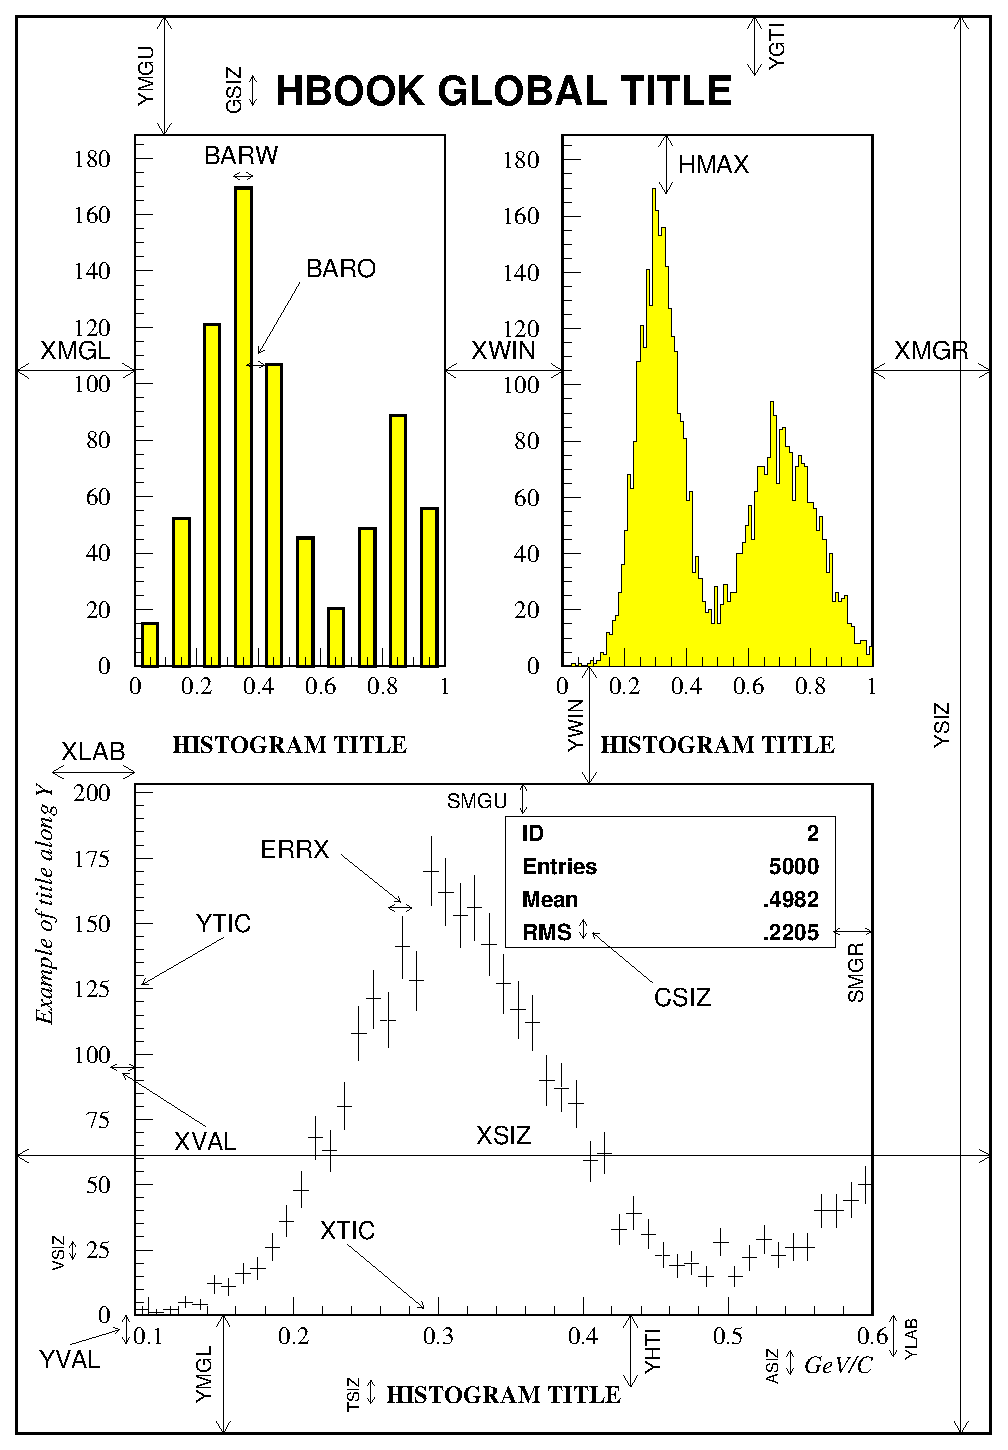
\epsfig{file=hplset.eps,width=14cm}}\end{center}
\caption{A graphical view of the {\tt SET} parameters}
\label{fig:HPLSET}
\end{figure}
\clearpage

\section{More on labels}
\index{alphanumeric!labels}
\index{label}

\begin{figure}
\begin{center}\mbox{\epsfig{file=ndvx.eps,width=16cm}}\end{center}
\caption{Example of labelling for horizontal axes}
\label{fig:LABNDVX}
\end{figure}

By default, labels used by \PAWcind{AXIS} and \PAWcind{PIE}
are numeric labels.
The command \PAWcind[LABELS]{GRAPHICS/PRIMITIVES/LABELS}
(or \PAWcind{LABELS} for short), allows the user to define
up to nine alphanumeric set of labels
(numbered from \texttt{1} to \texttt{9}).
These labels can then be used in subsequent commands
using \PAWcind{PIE} or \PAWcind{AXIS} primitives of HIGZ.

The \PAWcind{LABELS} command has three parameters:
\begin{DLtt}{123456}
\item[LABNUM] An integer between \texttt{1} and \texttt{9}.
              It identifies the labels set.
\item[NLABS]  The number of items to be placed on the labels 
              (up to \texttt{50}).
\item[CHLABS] \texttt{NLABS} character strings specifying the label items.
\end{DLtt}

\newpage

The label sets thus defined can be used for axes on all plots produced
by PAW (HPLOT histograms, graphs, vectors drawing, etc.) via the
\PAWcind[SET]{SET NDVX (NDVY)} command.
\index{axis!divisions}
These commands have the following structure:

\subsection*{Example of \texttt{NXDV} specification}
\begin{alltt}
    SET \Ssind{NDVX} i            e.g. SET NDVX 512
{\rm or}
    SET \Ssind{NDVX} i.jk         e.g. SET NDVX 10.25
\end{alltt}

In the first case the number \texttt{i} contains
\texttt{100} times the 
number of secondary divisions plus the number of primary divisions.
(e.g. \texttt{512} means \texttt{12} primary and \texttt{5} secondary division. 
By adding \texttt{10000} times \texttt{N3} to \texttt{i} a third level of divisions
is available.
\index{divisions}

In the second case the number in front of the dot \texttt{(i)} indicates the total
number of divisions, the first digit following the dot \texttt{(j)} the label
identifier (\texttt{LABNUM}) (if this number is equal to \texttt{0} numeric labels
are drawn). The second digit after the \texttt{(k)} dot indicates the position 
where the \index{label!text justification} labels have to be drawn (i.e. the
{\em text justification} parameter, in this case \texttt{5}, indicating 
horizontally written text centered on the interval). Study figures 
\ref{fig:LABNDVX} and \ref{fig:LABNDVY} for details. These two figures show 
that the labels can be centered on the tick marks (\texttt{1} to \texttt{4}) or on 
the divisions (\texttt{5} to \texttt{8}). If the labels are centered on the tick 
marks, note that the number of items in the command \texttt{LABELS} must be equal
to the number of tick marks (which is equal to the number of divisions 
{\bf plus one}), otherwise the last alphanumeric label on the axis will be 
undefined. \index{tick marks}

By default, the number of primary divisions given by \PAWcind[SET]{SET NDVX n}, 
\PAWcind[SET]{SET NDVY n} or \PAWcind[SET]{SET NDVZ n} is optimized to have a 
reasonable labelling. The number of primary divisions is also optimized 
according the number of zones (command \PAWcind[ZONE]{ZONE}) i.e : 
along the X direction the number of primary divisions is divided by 
\texttt{the_number_of_X _zones} along the Y direction the number of primary 
divisions in divided by \texttt{(the_number_of_Y_zones)/2}.

If the number of divisions has to be exactly equal to the
number given by \PAWcind[SET]{SET NDVX n}, \PAWcind[SET]{SET NDVY n} or
\PAWcind[SET]{SET NDVZ n}, a negative value must be used i.e.:
\subsection*{Forcing an exact number of divisions}
\begin{alltt}
    SET \Ssind{NDVX} -i            e.g. SET NDVX -512
or
    SET \Ssind{NDVX} -i.jk         e.g. SET NDVX -10.25
\end{alltt}

For example to label each subsequent X-axis with the names of the
months of the year centered in the middle of each bin one can use:
\subsection*{Example of alphanumeric labels on an axis}
\begin{alltt}
PAW > \Ucom{LABEL 1 12 JAN FEB MAR APR MAY JUN JUL AUG SEP OCT NOV DEC}
PAW > \Ucom{SET NDVX -12.15}
\end{alltt}

\begin{figure}[p]
\begin{center}\mbox{\epsfig{file=ndvy.eps,width=16cm}}\end{center}
\caption{Example of labelling for vertical axes}
\label{fig:LABNDVY}
\end{figure}

\section{Colour, line width, and fill area in HPLOT}
\index{histogram!presentation}
\index{fill!area}
\index{colour}
\index{line!width}

The aspect of HPLOT pictures can be modified via the \texttt{xWID}, \texttt{xTYP}
and \texttt{xCOL} attributes, where \texttt{x} can be \texttt{H}, \texttt{B},
\texttt{P}, or \texttt{F}, defined as follows:
\begin{DLtt}{12}
\item[B] zone Box
\item[F] Function
\item[H] Histogram
\item[P] Page
\end{DLtt}

The values given to the parameters \Ssind{PTYP}, \Ssind{BTYP}, \Ssind{HTYP},
and \Ssind{FTYP} are the HIGZ fill area interior styles. Interior style
 provided by the basic graphics package (i.e. GKS) can be used (cf the
corresponding documentation) but in order to have the same result on all 
devices, numbers greater than \texttt{100} (HIGZ styles: \ref{fig:HATCH}) should
be used. Figure \ref{fig:BTYP} shows how to use the \texttt{xTYP} parameter. 

The parameters \Ssind{PCOL}, \Ssind{BCOL}, \Ssind{HCOL} and \Ssind{FCOL}
are equivalent to \Ssind{PTYP}, \Ssind{BTYP}, \Ssind{HTYP}, and \Ssind{FTYP}
respectively, but instead of changing the hatch style, they change the
colour of the same areas. It is possible to specify both the border and
the inside color for the Histogram, Box Page, and Function (\Ssind{HCOL}, 
\Ssind{BCOL}, \Ssind{PCOL}, \Ssind{FCOL}).
\subsection*{Example of \texttt{HCOL} specification}
\begin{alltt}
      Ex:
                  +---- 1 The Histogram is filled
                  |     0 Only the border is drawn 
                  |+--- Border color (here 2) if the histogram is filled
                  ||++- Inside color (here 3) if the histogram is filled
                  ||||  Border color if the histogram is not filled
                  ||||
                  VVVV
       SET  HCOL  1203  
\end{alltt}
The same mechanism is also available for \Ssind{FCOL}, \Ssind{BCOL} and 
\Ssind{PCOL}.

If \Ssind{PCOL}, \Ssind{BCOL}, \Ssind{HCOL} or \Ssind{FCOL} are between \texttt{1}
and \texttt{99}, then only the contour of the corresponding area is changed. 
If they are between \texttt{1001} and \texttt{1099}, then the surface is filled with
the colour determined by the corresponding fill area colour index (1 to 99).
If they are between \texttt{1199} and \texttt{1999}, then the surface is filled with
the colour determined by the corresponding fill area colour index (1 to 99)
and the border is drawn with the corresponding line color index (1 to 9).

If one of the \Ssind{*COL} is greater than 1000 the corresponding value of the
Fill Area Interior Style (for \Ssind{HTYP}, \Ssind{BTYP}, \Ssind{PTYP} or 
\Ssind{FTYP}) is automatically set to \texttt{1} (solid).

In addition, \Ssind{BCOL} has two digits after the dot. The first one specifies
the colour of the zone box shadowing and the second the colour
of the statistic box shadowing. 
\index{colour}

\begin{figure}[p]
\begin{center}\mbox{\epsfig{file=btyp.eps,width=16cm}}\end{center}
\caption{Usage of fill area types in HPLOT}
\label{fig:BTYP}
\end{figure}
\clearpage

\section{Information about histograms}
\index{date!and hour on pictures}
\index{file name!on pictures}
\index{date}
\index{fit!parameters on pictures}
\index{statistic!parameters on pictures}

Four options are available to plot additional informations on HPLOT pictures:
\Oind{DATE}, \Oind{FILE}, \Oind{STAT} and \Oind{FIT}.

\begin{alltt}
PAW > \Ucom{OPTION DATE}        | Plot date and hour on current HPLOT picture
PAW > \Ucom{OPTION FILE}        | Plot file name of current histogram
PAW > \Ucom{OPTION STAT}        | Plot statistics of current histogram
PAW > \Ucom{OPTION FIT}         | Plot Fit parameters of current histogram
\end{alltt}

For each of these \PAWcind{OPTION} commands a corresponding 
\PAWcind{SET} parameter is available:

\begin{alltt}
PAW > \Ucom{SET DATE i}    | Default is 2
PAW > \Ucom{SET \Ssind{FILE} i}    | Default is 1
\end{alltt}
where \texttt{i} defines the position of the date or file name:

\begin{DLtt}{12345678}
\item[i = 1 :] Top left corner        of page/current histogram.
\item[i = 2 :] Top right corner
\item[i = 3 :] Bottom left corner
\item[i = 4 :] Bottom right corner
\end{DLtt}

For example the command:
\begin{alltt}
PAW > \Ucom{SET \Ssind{DATE} 3}
\end{alltt}
sets the position of the date to the bottom left corner of the HPLOT pictures.
\begin{alltt}
PAW > \Ucom{SET \Ssind{STAT} i}    | Default is 1111
\end{alltt}
where \texttt{i} corresponds to binary status bits \texttt{AOURMEI} as follows: 

\begin{DLtt}{1234}
\item[A=1] Draw the contents of all channels
\item[O=1] Draw number of overflows
\item[U=1] Draw number of underflows
\item[R=1] Draw R.M.S.
\item[M=1] Draw mean value
\item[E=1] Draw number of entries
\item[I=1] Draw histogram identifier
\end{DLtt}

For example the command:

\begin{alltt}
PAW > \Ucom{SET STAT 10}
\end{alltt}

sets the statistics informations to be only the number of entries.

\begin{alltt}
PAW > \Ucom{SET \Ssind{FIT} i}     | Default is 101
\end{alltt}
where \texttt{i} corresponds to binary status bits \texttt{CEP} as follows: 

\begin{DLtt}{123}
\item[C=1] Draw \(\chi^2\)
\item[E=1] Draw errors
\item[P=1] Draw fit parameters
\end{DLtt}

For example to draw only the result of the \(\chi^2\) fit one would use:
\begin{alltt}
PAW > \Ucom{SET FIT 100}
\end{alltt}

For all these \PAWcind{OPTION}s, the {\bf character size} is specified with the 
command \PAWcind[SET]{SET CSIZ} and the character font used with 
\PAWcind[SET]{SET CFON}.



\subsection*{Fill area style, marker and line type}

The Fill Area Interior Style, The Fill Area Style Index,
the Marker TYPe and the Line TYPe are set respectively using the
\PAWcind{IGSET} parameters
\Ssind{FAIS}, \Ssind{FASI}, \Ssind{MTYP} and \Ssind{LTYPE}.

\subsection*{Example}
\begin{alltt}
PAW > \Ucom{IGSET FAIS 3}      | Fill area are hatched
PAW > \Ucom{IGSET FASI 244}    |   with the style index
PAW > \Ucom{IGSET MTYP 25}     | Marker type is an empty square
PAW > \Ucom{IGSET LTYP 15}     | Line type is dotted
\end{alltt}
\index{hatch style}
\index{fill!area!style index}
\index{fill!area!interior style}
\index{marker!type}
\index{line!type}

HIGZ provides some portable fill area styles index coded
using three digits \texttt{ijk} as follows:

\begin{DLtt}{12}
\item[i:] Distance between each hatch in mm
\item[j:] Angle between \texttt{90} and \texttt{180} degrees
\item[k:] Angle between \texttt{0} and \texttt{90} degrees
\end{DLtt}

These numbers are coded according to table \ref{tab:HIGZSTY}
and examples are shown in figure \ref{fig:HATCH}.

\begin{table}
\[
\begin{array}{|crcrcr|}
\hline
\mbox{\tt i} &  \mathrm{Distance} &
\mbox{\tt j} &  \mathrm{Angle}    &
\mbox{\tt k} &  \mathrm{Angle}     \\
\hline
   &                               &
0  & 180^{\circ}                   &
0  &   0^{\circ}                   \\
1  & 0.75 \mathrm{mm}              &
1  & 170^{\circ}                   &
1  &  10^{\circ}                   \\
2  & 1.50 \mathrm{mm}              &
2  & 160^{\circ}                   &
2  &  20^{\circ}                   \\
3  & 2.25 \mathrm{mm}              &
3  & 150^{\circ}                   &
3  &  30^{\circ}                   \\
4  & 3.00 \mathrm{mm}              &
4  & 135^{\circ}                   &
4  &  45^{\circ}                   \\
5  & 3.75 \mathrm{mm}              &
5  & \multicolumn{1}{c}{\mbox{not drawn}} &
5  & \multicolumn{1}{c|}{\mbox{not drawn}} \\
6  & 4.50 \mathrm{mm}              &
6  & 120^{\circ}                   &
6  &  60^{\circ}                   \\
7  & 5.25 \mathrm{mm}              &
7  & 110^{\circ}                   &
7  &  70^{\circ}                   \\
8  & 6.00 \mathrm{mm}              &
8  & 100^{\circ}                   &
8  &  80^{\circ}                   \\
9  & 6.75 \mathrm{mm}              &
9  &  90^{\circ}                   &
9  &  90^{\circ}                   \\
\hline
\end{array}
\]
\caption{Codification for the HIGZ portable fill area interior styles}
\label{tab:HIGZSTY}
\end{table}

\subsection*{Example}
\begin{alltt}
PAW > \Ucom{IGSET FAIS 3}      | Fill area interior style is hatched
PAW > \Ucom{IGSET FASI 190}    | Hatch type is 190
\end{alltt}
These commands will yield hatching with two sets of lines
at $90^{\circ}$ and $0^{\circ}$ spaced 1 mm apart.

\begin{figure}[p]
\begin{center}\mbox{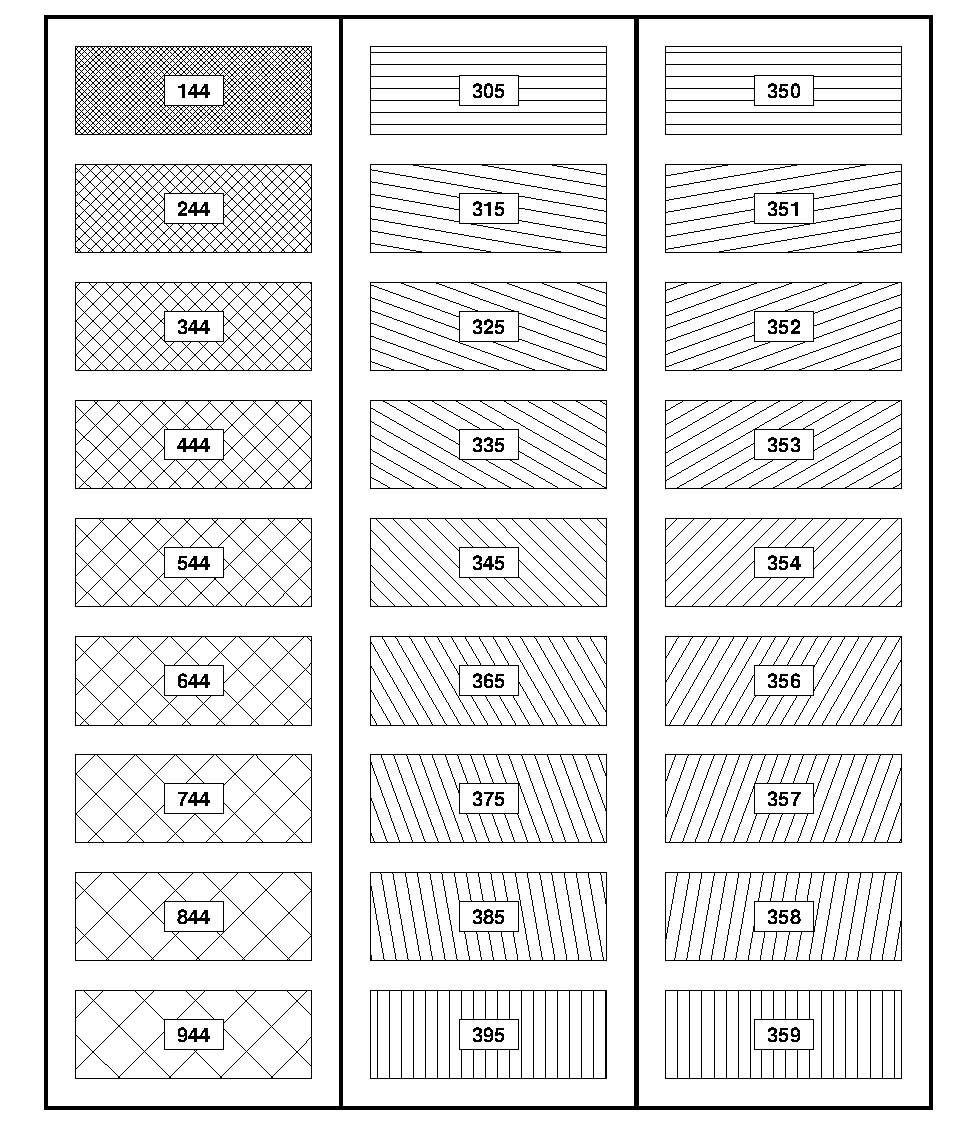
\epsfig{file=fasi.eps,width=16cm}}\end{center}
\caption{HIGZ portable hatch styles}
\label{fig:HATCH}
\index{hatch style}
\end{figure}

\begin{figure}[p]
\begin{center}\mbox{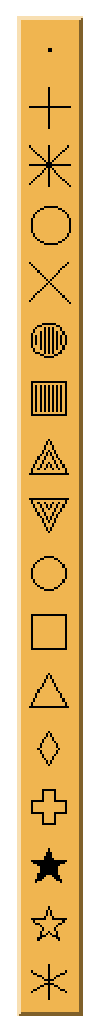
\epsfig{file=marker.eps,width=12cm}}\end{center}
\caption{HIGZ portable marker types}
\label{fig:MTYPE}
\index{marker!type}

\begin{center}\mbox{\epsfig{file=ltype.eps,width=12cm}}\end{center}
\caption{HIGZ portable line types}
\label{fig:LTYPE}
\index{line!type}
\end{figure}

\begin{figure}
\epsfig{file=greylev.eps,width=\textwidth}
\caption{PostScript grey level simulation of the basic colours}
\label{fig:GREYLEV}
\index{fonts}
\end{figure}

\clearpage


\section{Text drawing}
In PAW, text output can be produced in two ways:
\begin{enumerate}
\item {\em Automaticaly} with commands like \PAWcind{GRAPH} or 
      \PAWcind{HISTO/PLOT} in which a lot of text is drawn: the axis labels, the
      histogram title, the global title, the statistics etc. . The attributes
      (font, colour or size) and the placement of these texts are controled 
      with the command \PAWcind{SET}. In the rest of the chapter, the text
      produce {\em automaticaly} will be called {\em HPLOT text}
\item {\em Directly} with the commands \PAWcind{ITX} and \PAWcind{TEXT}. The 
      attributes of \PAWcind{ITX} are controlled with the command 
      \PAWcind{IGSET} whereas the attributes of \PAWcind{TEXT} are given
      with the command parameters.
\end{enumerate}

\subsection*{Text placement}
The text placement specify where the text must be drawn. For the
{\em HPLOT text}, the text position  is always in centimeters whereas for
\PAWcind{ITX} or \PAWcind{TEXT} the current coordinate system is used. 
\subsubsection{HPLOT text}
The possible text placements for {\em HPLOT text} are described in the
following example:
\begin{alltt}
PAW > \Ucom{SET XVAL 0.40} | distance between the Y axis and the axis values
PAW > \Ucom{SET YVAL 0.20} | distance between the X axis and the axis values
PAW > \Ucom{SET YLAB 0.80} | distance X axis to labels
PAW > \Ucom{SET XLAB 1.40} | distance Y axis to labels
PAW > \Ucom{SET YGTI 1.50} | Y position of global title
PAW > \Ucom{SET YHTI 1.20} | Y position  of histogram title
PAW > \Ucom{SET YNPG 0.60} | Y position for the page number
PAW > \Ucom{HISTO/PLOT 10} | the histogram 10 is drawn with previous settings
\end{alltt}
See figure \ref{fig:HPLSET} for more details.
\subsubsection{ITX}
In the command \PAWcind{ITX} the text position is defined with two mandatory
parameters (\texttt{X} and \texttt{Y}): 
\begin{alltt}
PAW > \Ucom{SELNT 1}         | cm coordinates
PAW > \Ucom{ITX 5 5 'Hello'} | 'Hello' is drawn at the position (5,5)
\end{alltt}
\subsubsection{TEXT}
In the command \PAWcind{TEXT} the text position is defined with two mandatory
parameters (\texttt{X} and \texttt{Y}): 
\begin{alltt}
PAW > \Ucom{SELNT 1}            | cm coordinates
PAW > \Ucom{TEXT 5 5 'Hello' 1} | 'Hello' is drawn at the position (5,5)
\end{alltt}

\subsection*{Text size}
For all the texts drawn with PAW commands, the text size is always specified
in centimeters.
\subsubsection{HPLOT text}
The possible text sizes for {\em HPLOT text} are described in the
following example:
\begin{alltt}
PAW > \Ucom{SET ASIZ 0.28} | axis label size
PAW > \Ucom{SET CSIZ 0.28} | comment size
PAW > \Ucom{SET GSIZ 0.28} | global title size
PAW > \Ucom{SET KSIZ 0.28} | Hershey character size
PAW > \Ucom{SET 2SIZ 0.28} | scatter plot and table character. size
PAW > \Ucom{SET TSIZ 0.28} | histogram title size
PAW > \Ucom{SET VSIZ 0.28} | axis values size
PAW > \Ucom{HISTO/PLOT 10} | the histogram 10 is drawn with previous settings
\end{alltt}
See figure \ref{fig:HPLSET} for more details.
\subsubsection{ITX}
The text character heigh attribute for use by future invocations of 
\PAWcind{ITX} is set using the \Ssind{CHHE} parameter as follows:
\begin{alltt}
PAW > \Ucom{IGSET CHHE 1}    | set the character heigh to 1 cm.
PAW > \Ucom{ITX 5 5 'Hello'} | the size of 'Hello' is 1 cm.
\end{alltt}
\subsubsection{TEXT}
In the command \PAWcind{TEXT} the text size is a mandatory parameter
(\texttt{SIZE}).
\begin{alltt}
PAW > \Ucom{TEXT 5 5 'Hello' 1} | the size of 'Hello' is 1 cm.
\end{alltt}

\subsection*{Text orientation}
The text orientation is an angle (in degrees) between the \texttt{X} axis
and the text axis. By default this angle is equal to 0.
\subsubsection{HPLOT text}
Text orientation cannot be changed with some \PAWcind{SET} parameters for the
{\em HPLOT text}. It is always automaticaly computed. For example in
the command \PAWcind{ATITLE}, which draws the axis titles, the title
on the \texttt{Y} axis is automaticaly drawn with an angle of 90 degrees.
\subsubsection{ITX}
The text orientation attribute for use by future invocations of 
\PAWcind{ITX} is set using the \Ssind{TANG} parameter as follows:
\begin{alltt}
PAW > \Ucom{IGSET TANG 90}   | set the text angle to 90 degrees.
PAW > \Ucom{ITX 5 5 'Hello'} | 'Hello' is drawn with an angle of 90 degrees.
\end{alltt}
\subsubsection{TEXT}
In the command \PAWcind{TEXT} the text orientation is an optional parameter
(\texttt{ANGLE}).
\begin{alltt}
PAW > \Ucom{TEXT 5 5 'Hello' ! 90} | 'Hello' is drawn with an angle of 90 degrees
\end{alltt}

\subsection*{Text alignment}
\index{text!alignment!horizontal}
\index{text!alignment!vertical}
The text alignment controls the placement of the character string  with 
respect to the specified text position.
\subsubsection{HPLOT text}
Text alignment cannot be changed for the
{\em HPLOT text}. It is automaticaly computed.
\subsubsection{ITX}
The text alignment attributes for use by future invocations of \PAWcind{ITX}
are set using the \Ssind{TXAL} parameter as follows:
\begin{alltt}
PAW > \Ucom{IGSET TXAL (10*(horizontal alignment) + (vertical alignment))}
\end{alltt}
The horizontal and 
vertical alignments parameters must be in the range \texttt{0-3}. The horizontal 
alignment specifies which end of the string (or its geometric center) is 
aligned with the specified point given in \PAWcind{ITX}.
The vertical alignment controls whether the top of tall characters
(or the bottom of capital letters) line up with the specified point 
(see figure \ref{fig:ALIGN}).
\begin{itemize}
\item[ITXALH] horizontal alignment
\begin{itemize}
\item[0] normal (usually same as 1)
\item[1] left end of string at specified point
\item[2] center of string at specified point
\item[3] right end of string at specified point
\end{itemize}
\item[ITXALH] vertical alignment
\begin{itemize}
\item[0] normal
\item[1] top of tallest chars plus any built in spacing
\item[2] top of tallest chars
\item[3] halfway between 2 and 4 
\end{itemize}
\end{itemize}
\begin{figure}
\begin{center}\mbox{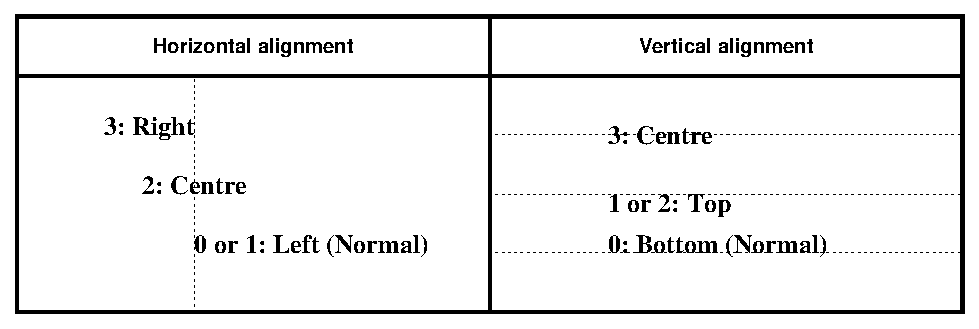
\epsfig{file=align.eps,width=16cm}}\end{center}
\caption{Text alignment}
\label{fig:ALIGN}
\index{text alignment}
\end{figure}
\begin{alltt}
PAW > \Ucom{IGSET TXAL 23}   | The horizontal and vertical alignments are centered
PAW > \Ucom{ITX 5 5 'Hello'} | 'Hello' is drawn center adjusted
\end{alltt}
\subsubsection{TEXT}
In the command \PAWcind{TEXT} the text aligment is an optional parameter
(\texttt{CHOPT}). Only the horizontal alignement can be changed among three 
possible values: Left, Center or Right.
\begin{alltt}
PAW > \Ucom{TEXT 5 5 'Hello' 1 ! L} | 'Hello' is drawn left adjusted (default)
PAW > \Ucom{TEXT 5 5 'Hello' 1 ! C} | 'Hello' is drawn center adjusted
PAW > \Ucom{TEXT 5 5 'Hello' 1 ! R} | 'Hello' is drawn right adjusted
\end{alltt}

\subsection*{Text colour}
The text colour is define via a colour index in the colour table.
\subsubsection{HPLOT text}
\begin{alltt}
PAW > \Ucom{SET XCOL 2}    | X axis color
PAW > \Ucom{SET YCOL 3}    | Y axis color
PAW > \Ucom{HISTO/PLOT 10} | the histogram 10 is drawn with previous settings
\end{alltt}
\subsubsection{ITX}
The text colour attribute for use by future invocations of 
\PAWcind{ITX} is set using the \Ssind{TXCI} parameter as follows:
\begin{alltt}
PAW > \Ucom{IGSET TXCI 3}    | set the text colour to green.
PAW > \Ucom{ITX 5 5 'Hello'} | 'Hello' is drawn in green.
\end{alltt}
\subsubsection{TEXT}
The text colour attribute for use by future invocations of 
\PAWcind{TEXT} is set using the \Ssind{TXCI} parameter as follows:
\begin{alltt}
PAW > \Ucom{IGSET TXCI 2}       | set the text colour to red.
PAW > \Ucom{TEXT 5 5 'Hello' !} | 'Hello' is drawn in red.
\end{alltt}

\subsection*{Text font and precision}
\index{font!text}
\index{text!font}
\index{text!precision}
\index{precision!text}
Text font selects the desired character font e.g. a roman font, a sans-serif 
font, etc. Text precision specifies how closely the graphics package 
implementation must follow the current size and orientation attributes. 
String (\texttt{0}) precision is most liberal (hardware), stroke (\texttt{2}) 
precision is most strict. Character precision is in the middle (\texttt{1}). 
The value of text font is dependent upon the basic graphics package used. 
However, font number \texttt{0}, with precision \texttt{2} is always available,
independently from the basic graphics package used.% (see figure \ref{fig:SOFT}).
Hardware characters are available with all the basic graphics packages. With
X11, a large variety of font is available. They are the same as the PostScript
fonts (see figure \ref{PS-FONT}).

\subsubsection{HPLOT text}
\begin{alltt}
PAW > \Ucom{SET CFON -60}  | comment font is Helvetica Bold
PAW > \Ucom{SET GFON -20}  | global title font is Times Bold
PAW > \Ucom{SET LFON -60}  | axis labels font is Helvetica Bold
PAW > \Ucom{SET TFON -20}  | general comments is Times Bold
PAW > \Ucom{SET VFON -60}  | axis values font is Helvetica Bold
PAW > \Ucom{HISTO/PLOT 10} | the histogram 10 is drawn with previous settings
\end{alltt}
Note that \texttt{SET *FON ffp} set all the {\em HPLOT text} font to the
same value \texttt{ffp}.

\subsubsection{ITX}
Text font and precision attributes for use by later
invocations of \PAWcind{ITX} are set with \Ssind{TXFP} as follows:
\begin{alltt}
PAW > \Ucom{IGSET TXFP (10*(Text font) + (text precision))}
\end{alltt}

\subsubsection{TEXT}
This command draws a software character text, independently from the basic
graphics package used by HIGZ. It can produce over 300 different graphic signs.
The way in which software characters are defined is via a string of valid
characters, intermixed by other characters, acting as ``escape'' characters
\index{character!escape} (e.g. a change of alphabet, upper or lower case). The
string is interpreted by \PAWcind{TEXT} and the resulting characters are 
defined according to the figure~\ref{SOFTTEXT}, which shows the list of 
available software characters. This command allows the user to mix different
types of characters (roman, greek, special, upper and lower case, sub and 
superscript). There are a total of 10 control characters.

\index{lower case letters}
\index{upper case letters}
\index{Greek letters}
\index{superscript}
\index{subscript}
\index{backspace}
\index{termination character}
\index{special symbols}
\label{ESCCHAR}
\begin{tabular}{||c|p{7cm}||c|p{7cm}||}
\hline
\multicolumn{4}{|c|}{\bf List of escape characters and their meaning}      \\
\hline
 $<$  & go to lower case                 & $>$  & go to upper case (default) \\
\hline
 \lsb & go to greek (Roman = default)    & \rsb & end of greek               \\
\hline
 "    & go to special symbols            & \#   & end of special symbols     \\
\hline
$\uparrow$  & go to superscript         & ?    & go to subscript            \\
\hline
 !    & go to normal level of script     & \&   & backspace one character    \\
\hline
 \$   & termination character (optional) &      &                            \\
\hline
\end{tabular}

Note that characters can be also entered directly in lower case or upper case
instead of using the control characters {\tt <} and {\tt >}.

The boldface characters may be simulated by setting the
attributes '\Sind{PASS}' and '\Sind{CSHI}' with \PAWcind{IGSET}.
The meaning of these attributes is the
following: Every stroke used to display the character is repeated
\Sind{PASS} times, at a distance (in percentage of the character height)
given by \Sind{CSHI}.

\clearpage

\begin{figure}
\begin{center}
\mbox{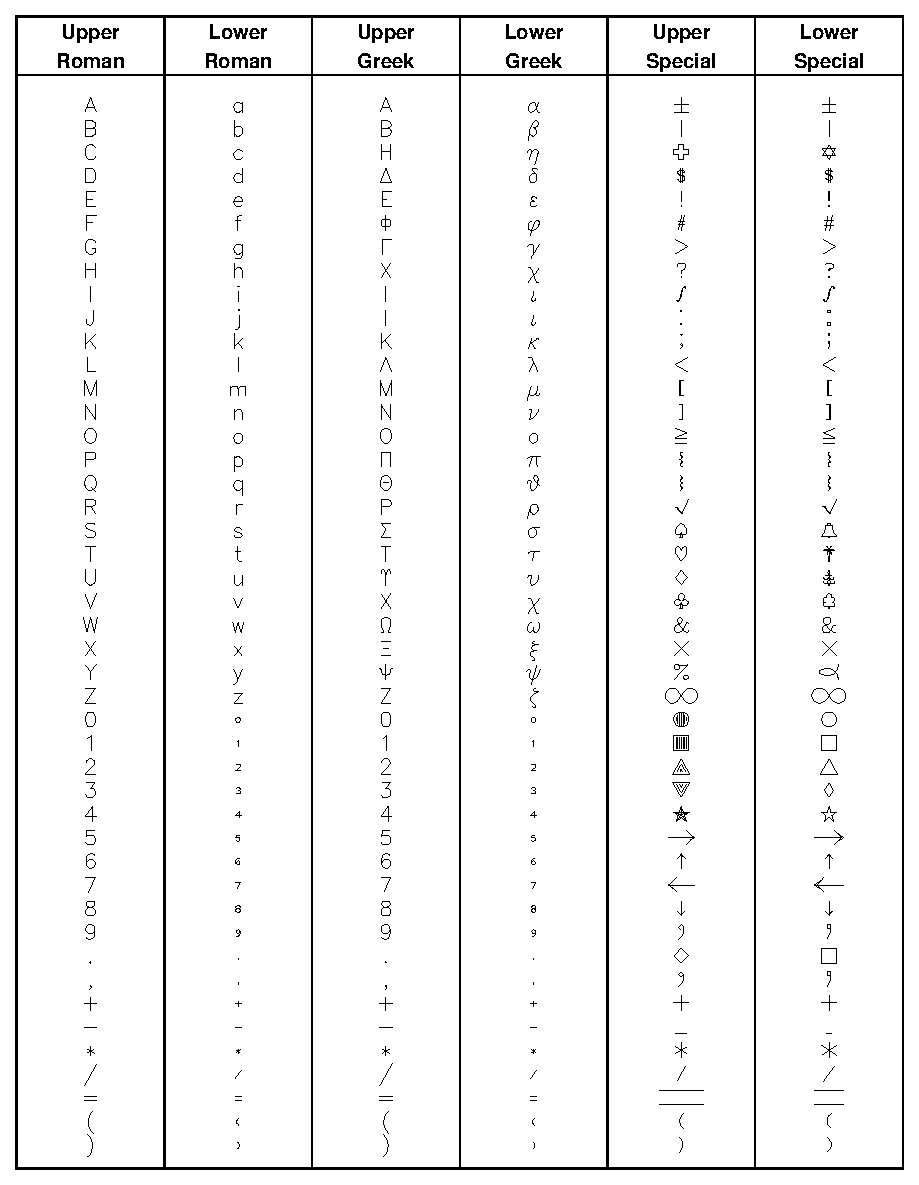
\epsfig{file=softtext.eps}}
\end{center}
\caption[Characters available in \texttt{IGTEXT}]%
        {Characters available in IGTEXT}
\label{SOFTTEXT}
\end{figure}

\clearpage

\subsubsection{PostScript text fonts}
\index{font!PostScript}
\index{PostScript!fonts}
\index{PostScript!fonts!Times-Italic}
\index{PostScript!fonts!Times-Bold}
\index{PostScript!fonts!Times-BoldItalic}
\index{PostScript!fonts!Helvetica}
\index{PostScript!fonts!Helvetica-Oblique}
\index{PostScript!fonts!Helvetica-Bold}
\index{PostScript!fonts!Helvetica-BoldOblique}
\index{PostScript!fonts!Courier}
\index{PostScript!fonts!Courier-Oblique}
\index{PostScript!fonts!Courier-Bold}
\index{PostScript!fonts!Courier-BoldOblique}
\index{PostScript!fonts!Symbol}
\index{PostScript!fonts!Times-Roman}
\index{PostScript!fonts!ZapfDingbats}

PostScript files the text can be generated with PostScript fonts. The figure 
\ref{PS-FONT} shows all the PostScript fonts available on most PostScript 
printers. Note that the fonts {\tt -15} to {\tt -24} are the same than 
{\tt -1} to {\tt -14}, but they are drawn in hollow mode.

The correspondence between ASCII and {\sf ZapfDingbats} font
is given on figures \ref{PSTEXT1} and \ref{PSTEXT2}.
\PAWcind{TEXT} control characters are taken into account. In addition
the character $\sim$ switches to the {\sf ZapfDingbats} character set.
\index{lower case letters}
\index{upper case letters}
\index{Greek letters}
\index{superscript}
\index{subscript}
\index{backspace}
\index{termination character}
\index{special symbols}
\begin{center}
\begin{tabular}{||c|l||c|l||}
\hline
\multicolumn{4}{|c|}{\bf List of escape characters and their meaning}      \\
\hline
 $<$  & go to lower case (optional)      & $>$  & go to upper case (optional)\\
\hline
 \lsb & go to greek (Roman = default)    & \rsb & end of greek               \\
\hline
 "    & go to special symbols            & \#   & end of special symbols     \\
\hline
$\sim$ & go to ZapfDingbats               & \#   & end of ZapfDingbats        \\
\hline
$\uparrow$  & go to superscript          & ?    & go to subscript            \\
\hline
 !    & go to normal level of script     & \&   & backspace one character    \\
\hline
 \$   & termination character (optional) &      &                            \\
\hline
\end{tabular}
\end{center}
\par
The PostScript fonts can be used with precision {\tt 0} or precision {\tt 1}.
On the screen, a PostScript font used with precision {\tt 1} appears
like the \PAWcind{TEXT} characters, with precision 0 its appears as
hardware character (X11 fonts). In both cases the  PostScript file is the same.

Note that characters can also be entered directly in lower or upper case
instead of using the escape characters {\tt <} and {\tt >}.

\subsection*{Example of PostScript text (result in figure
  \ref{PSEX1})}
\begin{alltt}
PAW > IGSET LWID 6
PAW > BOX 0 16 0 5 
PAW > IGSET CHHE 0.5
PAW > IGSET TXAL 3
PAW > IGSET TXFP -130
PAW > ITX 3 4 'K\bs{}355nstler in den gr\bs{}345\bs{}373ten st\bs{}311dten
PAW > ITX 3 3 '\bs{}253\bs{}265 l''\bs{}372uvre on conna\bs{}333t l''artisan\bs{}273
PAW > ITX 3 2 '\bs{}(proverbe fran\bs{}321ais\bs{}
PAW > ITX 3 1 '\bs{}252\bs{}241Ma\bs{}337ana\bs{}41 \bs{}322ag&\bs{}306!das&\bs{}313!\bs{}272, dit l''\bs{}323l\bs{}325ve.
\end{alltt}

\clearpage

\begin{figure}
\begin{center}\mbox{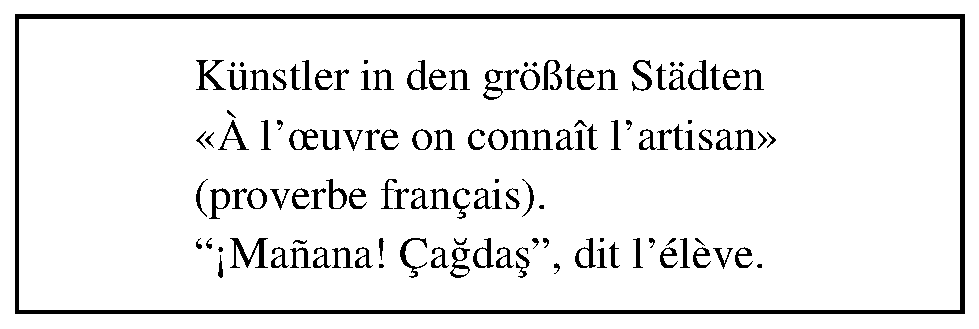
\epsfig{file=psex1.eps}}\end{center}
\caption{PostScript fonts usage (1).}
\label{PSEX1}
\end{figure}

\subsection*{Example of PostScript text and maths (result in figure
  \ref{PSEX2})}
\begin{alltt}
PAW > IGSET LWID 6
PAW > BOX 0 16 0 5
PAW > IGSET CHHE 0.5
PAW > IGSET TXAL 23
PAW > IGSET TXFP -130
PAW > ITX 8 4 'e^+!e^-! "5# Z^o! "5# ll&^-!, qq&^\bs{}261!'
PAW > ITX 8 3 '| a&^[\bs{}256]! \bs{}267 b&^[\bs{}256]! | = [\bs{}345] a^i?jk!+b^kj?i'
PAW > ITX(8 2 'i ("d#?[m!y]&^\bs{}261![g^m]! + m [y]&^\bs{}261! ) = 0" r# (~r# + m^2!) [y] = 0'
PAW > ITX 8 1 'L?em! = e J^[m]?em! A?[m]! , J^[m]?em!=l&^\bs{}261![ g?m]!l , M^j?i! = [\bs{}345&?a]! A?[a! t^a]j?i! '
\end{alltt}
\begin{figure}
\begin{center}\mbox{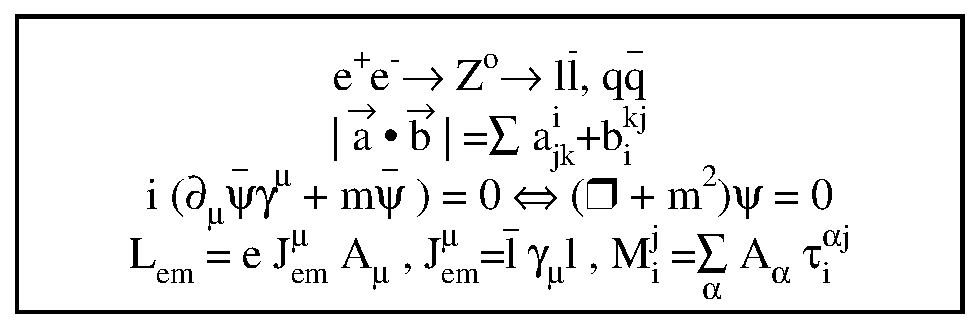
\epsfig{file=psex2.eps}}\end{center}
\caption{PostScript fonts usage (2).}
\label{PSEX2}
\end{figure}

\clearpage

\begin{figure}
\begin{center}\mbox{\epsfig{file=psfont.eps,width=\the\textwidth}}\end{center}
\caption{PostScript text fonts.}
\label{PS-FONT}
\end{figure}

\begin{figure}
\begin{center}\mbox{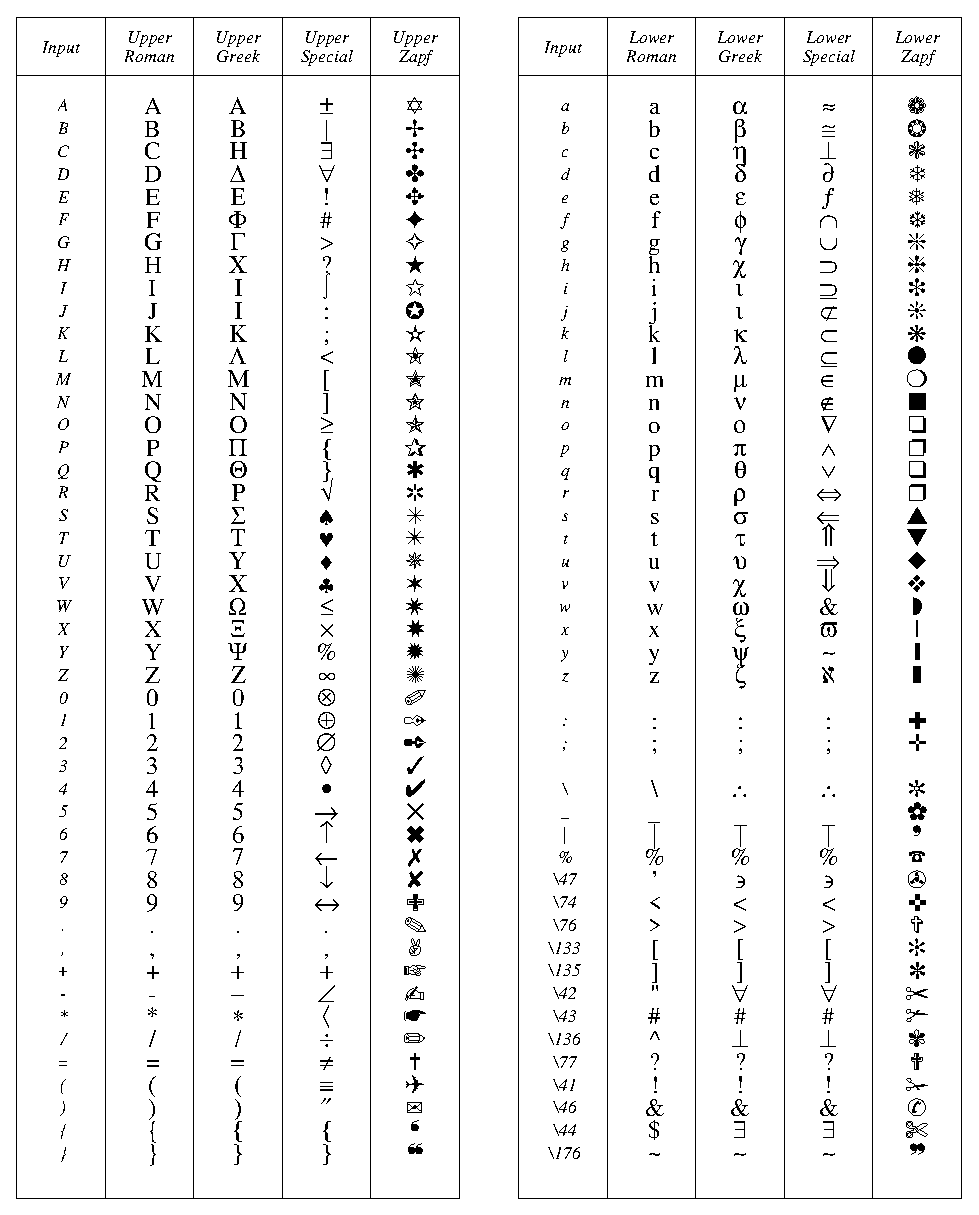
\epsfig{file=pstext1.eps,width=\the\textwidth}}\end{center}
\caption{PostScript characters (1).}
\label{PSTEXT1}
\end{figure}

\begin{figure}
\begin{center}\mbox{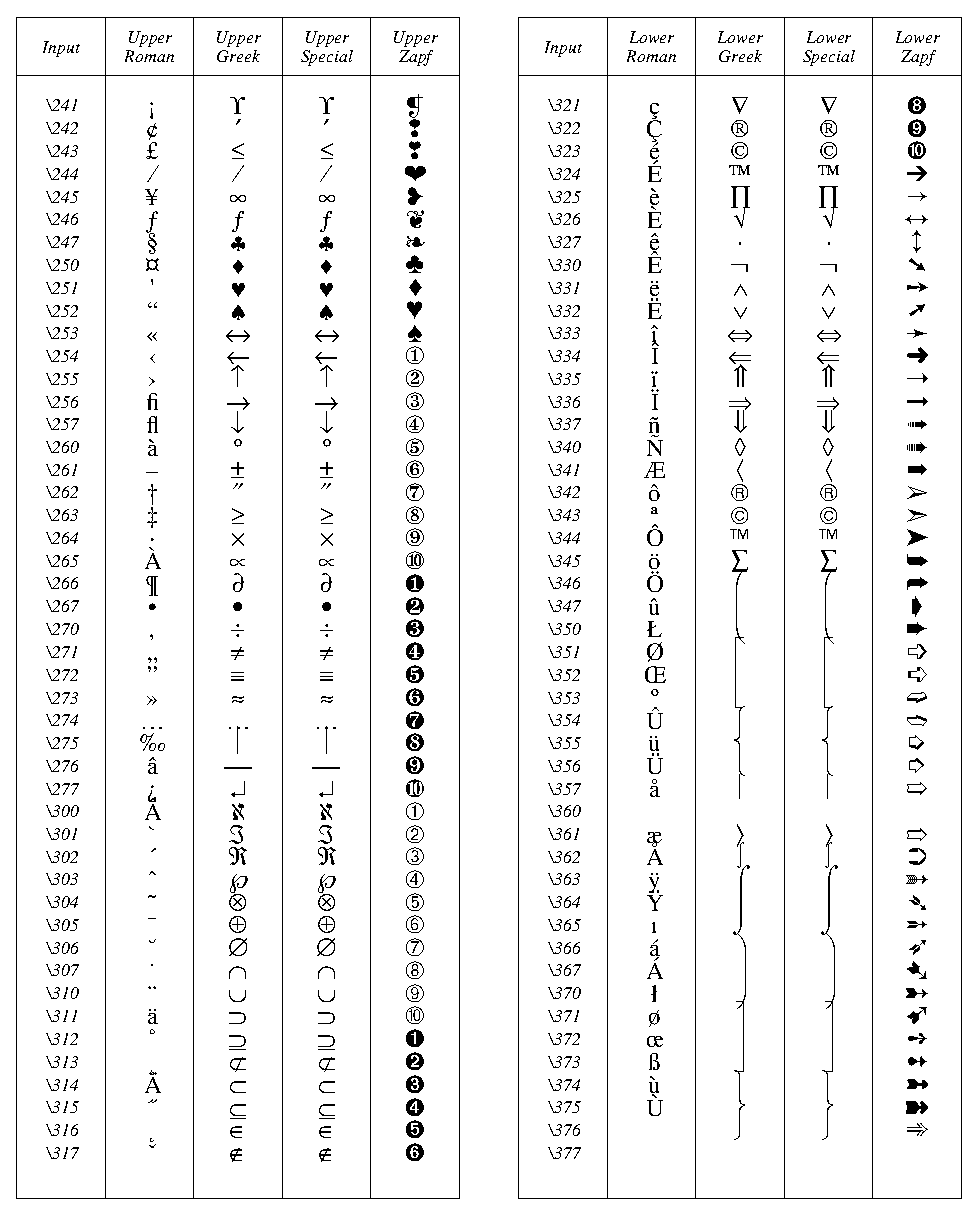
\epsfig{file=pstext2.eps,height=19cm}}\end{center}
\caption{PostScript characters (2).}
\label{PSTEXT2}
\end{figure}

\clearpage
\section{The HIGZ graphics editor}
\index{graphics!editor}
\index{editor}
\index{HIGZ!graphics editor}

The HIGZ pictures in memory can be modified interactively with the HIGZ
graphics editor. 
The command \PAWcind[MODIFY]{PICT/MODIFY} invokes the HIGZ editor
(see figure \ref{fig:GEDIFIG} for more details):
\begin{alltt}
PAW > \Ucom{PICT/MODIFY PNAME}
\end{alltt}
\texttt{PNAME} can be the complete name, the picture number in memory
or \texttt{' '}.

\begin{figure}
\includegraphics[width=\linewidth]{gedifig.eps}
\caption{The HIGZ graphics editor}
\label{fig:GEDIFIG}
\end{figure}
